\documentclass[crop, tikz, border=.1cm]{standalone}
\usetikzlibrary{positioning}
\usetikzlibrary{calc}
\usetikzlibrary{arrows.meta}
\begin{document}
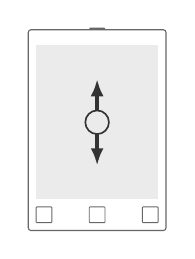
\begin{tikzpicture}
    \colorlet{border}{black!60}
\colorlet{screen}{black!8}
\colorlet{annotation}{black!80}

\newcommand\width{1.75}
\newcommand\height{2.55}
\newcommand\outborder{.1}
\newcommand\button{2 * \outborder}

\begin{scope}
    \tikzset{
        back slate/.style={
            border, fill=white,
            rounded corners=1,
        },
        lower key/.style={
            draw=border, line width=0.3, rectangle,
            rounded corners=0.25,
            minimum width={2 * \outborder cm},
            minimum height={2 * \outborder cm},
            inner sep=0pt,
        },
        upper key/.style={
            fill=border, rectangle,
            rounded corners=0.25,
            minimum width={2 * \outborder cm},
            minimum height=2pt,
            yshift=-.25pt,
            inner sep=0pt,
        },
    }

    \node[upper key] at (.5 * \width, \height) (key-t) {};
    \draw[back slate] (0, 0) rectangle (\width, \height);

    \fill[screen]
        (\outborder, 4 * \outborder)
        coordinate (screen-bl)
        rectangle (\width - \outborder, \height - 2 * \outborder)
        coordinate (screen-tr);

    \coordinate (screen-c) at ($(screen-bl)!.5!(screen-tr)$);

    \node[lower key] at (2 * \outborder, 2 * \outborder) (key-l) {};
    \node[lower key] at (.5 * \width, 2 * \outborder) (key-c) {};
    \node[lower key] at (\width - 2 * \outborder, 2 * \outborder) (key-r) {};
\end{scope}

    \newcommand\radius{.15}

    \draw[annotation, semithick] (screen-c) circle (\radius);
    \draw[annotation, ultra thick, -{Latex[length=2.2mm]}]
        ($(screen-c)+(0,\radius)$) -- ++(0, .4);

    \draw[annotation, ultra thick, -{Latex[length=2.2mm]}]
        ($(screen-c)-(0,\radius)$) -- ++(0, -.4);
\end{tikzpicture}
\end{document}
